%%%%%%%%%%%%%%%%%%%%%%%%%%%%%%%%%%%%%%%%%%%%%%%%%%%%%%%%%%%%%%%%%%%%%%%%
% Plantilla TFG/TFM
% Escuela Politécnica Superior de la Universidad de Alicante
% Realizado por: Jose Manuel Requena Plens
% Contacto: info@jmrplens.com / Telegram:@jmrplens
%%%%%%%%%%%%%%%%%%%%%%%%%%%%%%%%%%%%%%%%%%%%%%%%%%%%%%%%%%%%%%%%%%%%%%%%

\chapter{Estado del Arte}
\label{marcoteorico}

Antes de adentrarse en los detalles técnicos, es esencial establecer el contexto actual en el dominio de los buscadores multimedia basados en lenguaje natural. Esta revisión permitirá asentar una fundamentación teórica y metodológica sólida, comprender los desafíos y las limitaciones identificadas en investigaciones previas e identificar las brechas en el conocimiento existente, así como las oportunidades para realizar contribuciones significativas en LLMSearch.

\section{Modelos de Lenguaje Natural (LLMs) para Búsqueda}

Los \textbf{modelos de lenguaje de gran tamaño (LLMs)} han revolucionado el procesamiento del lenguaje natural en años recientes. Modelos como \emph{GPT-3} y \emph{GPT-4} (base de \textbf{ChatGPT}) demuestran que, con miles de millones de parámetros entrenados en enormes corpus de texto, es posible comprender y generar lenguaje con notable fluidez y contexto. Estos modelos capturan representaciones semánticas ricas, lo que habilita nuevas formas de \textbf{búsqueda semántica} y recuperación de información.

\textbf{Características clave:}

\begin{itemize}
  \item \textbf{Búsqueda por significado}: En lugar de limitarse a coincidencias de palabras clave, un LLM puede interpretar la intención de una consulta en lenguaje natural y relacionarla con documentos relevantes aunque no compartan palabras literalmente.
  
  \item \textbf{Embeddings semánticos}: Técnicas como \emph{embeddings} de oraciones (usando modelos tipo BERT o Sentence Transformers) convierten documentos y consultas a vectores en un espacio vectorial común, donde la similitud de coseno permite recuperar los contenidos más cercanos en significado.
  
  \item \textbf{Retrieval-Augmented Generation (RAG)}: Los LLMs pueden integrarse en pipelines donde primero se recuperan documentos candidatos y luego el modelo genera una respuesta o resumen usando esos textos.
  
  \item \textbf{Interfaz conversacional}: Modelos tipo ChatGPT permiten refinar iterativamente las consultas de búsqueda mediante diálogo, mejorando la precisión de resultados en consultas ambiguas.
\end{itemize}

Los avances más recientes se centran en mejorar la \textbf{eficiencia y apertura} de estos modelos. Mientras GPT-4 (de OpenAI) es de uso cerrado y con un tamaño muy grande no divulgado (>100B parámetros), han emergido modelos de código abierto como \emph{LLaMA} (Meta) y sus variantes, que con 7--70B parámetros logran desempeños competitivos.

\section{Modelos Visión-Lenguaje para Imágenes}

En un buscador multimedia, es esencial manejar consultas sobre contenido visual (imágenes) usando lenguaje natural. Aquí destacan los \textbf{modelos visiolingüísticos} o \textbf{modelos de visión-lenguaje (VLMs)}, que conectan representaciones de imágenes con representaciones textuales en un espacio común.

\subsection{CLIP y Embeddings Multimodales}

Un hito fue el modelo \textbf{CLIP} de OpenAI, que entrena conjuntamente un codificador de texto (transformer) y un codificador visual (Red Neuronal Convolucional o Visión Transformer) para proyectar ambos tipos de entrada en \textbf{vectores de embedding} de la misma dimensión. Mediante aprendizaje contrastivo en 400 millones de pares imagen--texto, CLIP logró que textos e imágenes con contenido semántico equivalente quedaran cercanos en el espacio vectorial.

\begin{figure}[h]
  \centering
  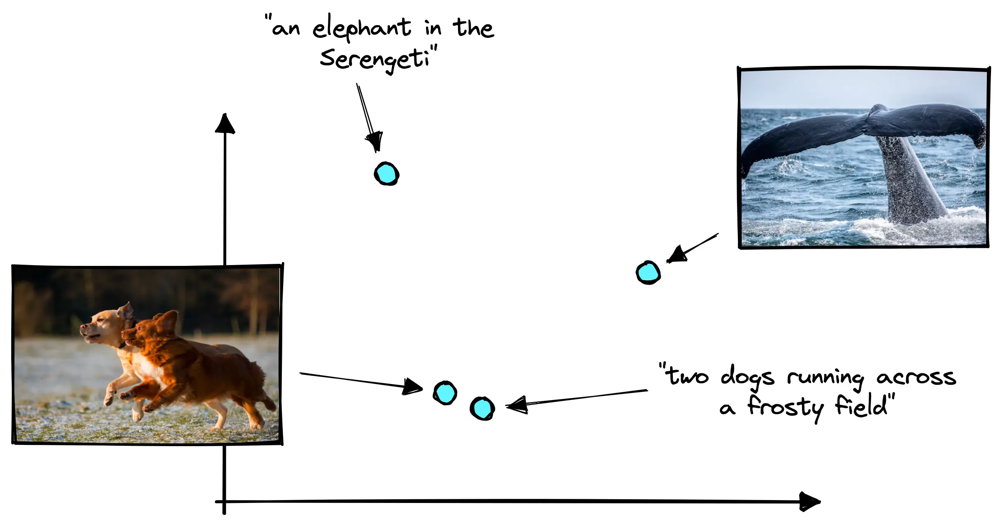
\includegraphics[width=0.7\textwidth]{archivos/clip_space.png}
  \caption{Ejemplo conceptual de un espacio vectorial multimodal entrenado por CLIP, donde imágenes y descripciones semánticas correspondientes se representan mediante vectores cercanos.}
  \label{fig:clip_space}
\end{figure}

\begin{figure}[h]
  \centering
  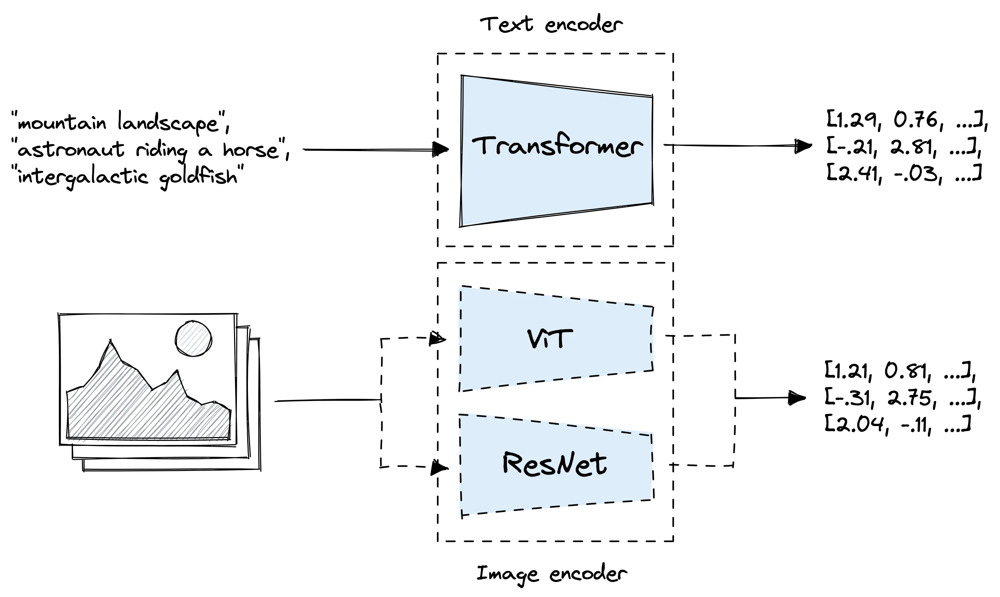
\includegraphics[width=0.7\textwidth]{archivos/clip_architecture.png}
  \caption{Arquitectura del modelo CLIP: encoder de texto y encoder de imagen que proyectan al mismo espacio de embedding.}
  \label{fig:clip_architecture}
\end{figure}

\subsection{Modelos Generativos de Descripción de Imágenes}

Otra línea de desarrollo son los \textbf{modelos generativos de descripción de imágenes}. Estos sistemas realizan \emph{image captioning}, es decir, generan en lenguaje natural una descripción para una imagen dada.

Modelos recientes como \textbf{BLIP-2} combinan:
\begin{itemize}
  \item Un encoder visual pre-entrenado (e.g. CLIP ViT)
  \item Un modelo de lenguaje grande congelado
  \item Un transformador ligero intermedio (Q-Former)
\end{itemize}

Esta arquitectura puentea la brecha visión-lenguaje eficientemente: el encoder de imagen extrae características visuales y el LLM genera la descripción textual.

\subsection{VQA y Diálogo Multimodal}

Junto con BLIP-2, han surgido numerosos modelos abiertos que permiten \textbf{Pregunta-Respuesta Visual (VQA)} y diálogo multimodal:

\begin{itemize}
  \item \textbf{LLaVA} (Large Language and Vision Assistant): Usa GPT-4 para generar datos sintéticos de entrenamiento y afina un modelo basado en \emph{Vicuna} (derivado de LLaMA) acoplado a un encoder visual.
  
  \item \textbf{Moondream}: Un VLM open-source de apenas 2 billones de parámetros (2B) que puede correr en tiempo real incluso en CPU o dispositivos móviles. Demuestra capacidades notables en:
  \begin{itemize}
    \item Generación de descripciones detalladas
    \item Respuesta a preguntas visuales
    \item Detección de objetos en modalidad cero-shot
    \item OCR básico (leer texto en imágenes)
  \end{itemize}
  
  \item \textbf{JoyCaption}: Un modelo de captioning de imágenes libre y sin censura, pensado originalmente para generar descripciones ricas que ayuden a entrenar modelos de difusión.
  
  \item \textbf{GPT-4 con visión} (GPT-4V): Demuestra capacidades impresionantes al responder con acierto a entradas que combinan imagen + texto, aunque su naturaleza propietaria limita su uso en entornos académicos.
\end{itemize}

\textbf{En síntesis}, el estado del arte en imagen+lenguaje ofrece dos enfoques complementarios para búsqueda multimedia:
\begin{enumerate}
  \item \emph{Embeddings} multimodales tipo CLIP para realizar \textbf{búsqueda directa por similitud} entre consultas textuales y contenido visual
  \item \emph{Modelos generativos visiolingüísticos} para \textbf{describir o entender imágenes en texto}, permitiendo indexar y razonar sobre imágenes mediante lenguaje natural
\end{enumerate}

\section{Modelos Multimodales para Vídeo}

Extender la búsqueda basada en lenguaje natural al dominio de \textbf{vídeo} conlleva retos adicionales, pues los vídeos combinan secuencias de imágenes con audio (y a veces texto incrustado).

\subsection{Técnicas de Procesamiento de Video}

\begin{enumerate}
  \item \textbf{Análisis por frames}: 
  \begin{itemize}
    \item Extraer fotogramas representativos del video
    \item Aplicar modelos de visión-lenguaje a cada frame
    \item Convertir el problema de vídeo a un conjunto de imágenes con marcas de tiempo
  \end{itemize}

  \item \textbf{Procesamiento de audio}:
  \begin{itemize}
    \item Usar modelos de \textbf{Reconocimiento Automático de Voz (ASR)} como \emph{Whisper}
    \item Transcribir con alta calidad el diálogo o narración presente en videos
    \item Indexar cada video por su transcripción textual completa
  \end{itemize}

  \item \textbf{Modelos video-texto end-to-end}:
  \begin{itemize}
    \item \emph{VideoCLIP}: Extiende la idea de CLIP al dominio temporal
    \item Transformers específicos para vídeo que realizan \emph{video captioning}
  \end{itemize}
\end{enumerate}

\subsection{Arquitecturas para Búsqueda en Video}

Una arquitectura emergente es combinar los enfoques anteriores en un pipeline RAG multimodal:
\begin{itemize}
  \item Indexar por un lado los \emph{frames} visuales mediante embeddings
  \item Indexar por otro lado las transcripciones de voz como texto
  \item Ante una consulta, recuperar fragmentos candidatos por similitud visual o textual
  \item Usar un modelo de lenguaje para sintetizar ambas fuentes y determinar la respuesta
\end{itemize}

\subsection{Modelos Unificados Multimodales}

\begin{itemize}
  \item \textbf{MiniGPT-4}: Acepta secuencias de imágenes como entrada (simulando un video corto)
  \item \textbf{MiniCPM-V}: Soporta entradas de video, generando una descripción general
  \item \textbf{Gemini} (Google): Integra visión, video y sonido en un mismo LLM
  \item \textbf{ImageBind} (Meta): Aprende una representación común para imágenes, texto, audio y otros sensores
\end{itemize}

\section{Análisis de Audio y Búsqueda mediante Sonido}

Para completar un buscador verdaderamente multimedia, se debe considerar contenido \textbf{audio} (fuera de videos, es decir, archivos de sonido o música).

\subsection{Procesamiento de Habla}

\begin{itemize}
  \item Si el audio es habla (podcasts, grabaciones, conferencias), aplicar \textbf{ASR} con modelos como Whisper
  \item Obtener una transcripción textual que se convierte en texto indexable
  \item Permitir búsquedas por palabras clave o semántica usando LLMs o embeddings
\end{itemize}

\subsection{Audio No Verbal}

Para audio que no es voz (sonidos ambientales, música, efectos sonoros):
\begin{itemize}
  \item \textbf{CLAP (Contrastive Language-Audio Pretraining)}: Entrena un encoder de audio y uno de texto conjuntamente
  \item Permite buscar efectos de sonido a partir de descripciones textuales
  \item Facilita la clasificación cero-shot de audio
\end{itemize}

\subsection{Modelos Generadores de Descripciones Auditivas}

\begin{itemize}
  \item \textbf{AudioCaption} (Microsoft): Genera frases descriptivas de clips de audio
  \item Permite describir cada audio en texto y luego indexar esas descripciones
  \item Facilita un acceso más semántico a archivos de sonido
\end{itemize}

\section{Comparativa de Modelos Representativos}

\begin{table}[h]
  \centering
  \resizebox{\textwidth}{!}{%
    \begin{tabular}{llll}
      & Modalidades                         & Tamaño     & Características principales                                                              \\ \hline
      ChatGPT (GPT-4)  & Texto (y visión en GPT-4V)         & >100 B?    & LLM propietario de OpenAI, rendimiento puntero en comprensión y generación de lenguaje. \\
      MiniCPM-V 2.5    & Texto, Imágenes, Vídeo, Audio      & ∼8 B       & Open-source, eficiente para despliegue en dispositivos; consultas multimodales.         \\
      Moondream 2      & Imágenes–Texto                     & 2 B        & VLM ultraligero con VQA, captioning, detección y OCR en CPU en tiempo real.           \\
      Whisper          & Audio–Texto                        & ∼1.6 B     & ASR multilingüe de código abierto, muy robusto ante acentos y ruido.                   \\ \hline
    \end{tabular}%
  }
  \caption{Comparativa de modelos representativos en lenguaje y multimodalidad.}
  \label{tab:comparativa_modelos}
\end{table}

En la tabla se observa la distinción entre modelos propietarios (e.g. ChatGPT) y una diversidad de iniciativas abiertas. Para \textbf{LLMSearch}, los módulos open-source (MiniCPM-V, Moondream, Whisper, CLAP, etc.) pueden combinarse para construir un sistema completo:
\begin{itemize}
  \item Transcripción de audio con Whisper
  \item Indexado de sonidos con CLAP
  \item Descripción de imágenes con Moondream o BLIP-2
  \item Orquestación conversacional con un LLM general (Vicuna/LLaMA)
\end{itemize}

\section{Conclusión}

El estado del arte ofrece los bloques fundamentales para un buscador multimedia por lenguaje natural. Este TFG integrará y adaptará estas tecnologías de vanguardia en una única plataforma unificada (\emph{LLMSearch}), evaluando su rendimiento y proponiendo mejoras para lograr búsquedas multimodales más precisas y naturales.